\ifdefined\iscombined
	\problemset{Problem Set 1}
\else
\documentclass{article}
\usepackage{xparse}
\usepackage{tabularx}
\usepackage{changepage}
\usepackage{listings}
\usepackage{amsthm}
\usepackage{comment}
\usepackage{amsmath}
\usepackage{braket}
\usepackage{amsfonts}
\usepackage{amssymb}
\usepackage{sectsty}
\usepackage{hyperref}
\usepackage{fancyhdr}
\usepackage[top=1in,bottom=1in,left=1in,right=1in]{geometry}
\usepackage{float}
\usepackage{graphicx}
\usepackage{mathtools}
\usepackage{tikz}
\usetikzlibrary{arrows}

\date{
	\vspace{-.75em}
	{\large \today}
}

\title{
	\vspace*{-1.5em}
	{\Huge Problem Set 1} \\
	\vspace{-1em}
	\rule{\textwidth/2}{.01em} \\
	\vspace{-.75em}
}

\author{
	{\large Matthew Farah}
}

\hypersetup{
	colorlinks=true,
	linkcolor=blue,
	filecolor=magenta,
	urlcolor=blue,
	citecolor=blue,
	anchorcolor=blue
}

\fancyhead{}
\fancyhead[L]{\today}
\fancyhead[R]{Problem Set 1}

\setlength{\parindent}{0cm}

\tikzset{vertex/.style = {shape = circle, draw, minimum size = 2em}}
\tikzset{edge/.style = {->,> = latex'}}

\newenvironment{solution}{
	\vspace{.5em}
	\par
	\begin{adjustwidth}{1.5em}{}
	\textbf{{Solution:}}
	\par
	\vspace{.5em}
}{
	\vspace{1em}
	\end{adjustwidth}
	\setcounter{step}{0}
}

\makeatother
\makeatletter

\newcounter{step}
\renewcommand{\thestep}{\Roman{step}}

\newenvironment{step}{
	\refstepcounter{step}
	\vspace{1em}\par\noindent
	\ignorespaces\noindent\textbf{(\thestep)}
	\ignorespaces
}{
	\par
	\vspace{1.5em}
}

\newcounter{problem}
\renewcommand{\theproblem}{\arabic{problem}}

\newenvironment{problem}[1][]{
	\newpage
	\refstepcounter{problem}
	\setcounter{subproblem}{0}
	\vspace{.5em}\par\noindent
	\begin{adjustwidth}{1.5em}{}
	\noindent\textbf{Problem \theproblem: }\noindent\textit{#1}
	\par
	\phantomsection
	\addcontentsline{toc}{section}{\protect{\large{Problem \theproblem}}}
}{
	\vspace{.5em}
	\end{adjustwidth}
}


\newcounter{subproblem}
\renewcommand{\thesubproblem}{\alph{subproblem}}

\newenvironment{subproblem}{
	\setcounter{step}{0}
	\refstepcounter{subproblem}
	\phantomsection
	\addcontentsline{toc}{subsection}{\protect{\large{(\thesubproblem)}}}
	\begin{adjustwidth}{1.5em}{}
	\noindent{\textbf{(\thesubproblem) }}\ignorespaces
}{
	\par
	\vspace{.5em}
	\end{adjustwidth}
}

\newcounter{lemma}
\renewcommand{\thelemma}{\arabic{lemma}}

\newenvironment{lemma}[1][]{
	\refstepcounter{lemma}
	\vspace{1em}\par\noindent
	\noindent\textbf{Lemma ({#1}): }\noindent\ignorespaces
}{
	\vspace{.5em}
}

\newcounter{proposition}
\renewcommand{\theproposition}{\arabic{proposition}}

\newenvironment{proposition}{
	\refstepcounter{proposition}
	\vspace{1em}\par\noindent
	\noindent\textbf{Proposition:}
	\noindent\textit
	\ignorespaces
}{
	\vspace{.5em}
}

\newcommand{\supp}[1]{\text{supp}({#1})}
\newcommand{\ord}[1]{\text{ord}({#1})}
\newcommand{\gen}[1]{\langle {#1} \rangle}
\newcommand{\lcm}[2]{\text{lcm}({#1}, {#2})}
\renewcommand{\mod}[1]{\ (\text{mod} \; {#1})}

\sectionfont{\fontsize{12}{12}\bfseries}
\subsectionfont{\fontsize{10}{12}\normalfont}
\subsubsectionfont{\fontsize{10}{12}\normalfont}

\begin{document}

\maketitle
\pagestyle{fancy}

\newcolumntype{Y}{>{\centering\arraybackslash}X}

\tableofcontents

\fi

\begin{problem}
	Goofus, a MAT102 student, has asked you to critique his proof. \\

	\fbox{
		\begin{minipage}{\dimexpr\linewidth-2\fboxsep-2\fboxrule\relax}
			\begin{proposition}
				Let $n \in \mathbb{Z}$. Then $n$ is odd if and only if $n^2$ is odd.
			\end{proposition}
		
			\begin{proof}
				$n$ odd $\implies \exists k, n = 2k + 1 \implies n^2 = (2k + 1)^{2} = 4k^{2} + 4k + 1 = 2(2k^{2} + 2k) + 1 = 2l + 1 \implies n^2$ odd. \\
		
				$n$ even $\implies n = 2k \implies n^{2} = (2k)^{2} = 4k^{2} = 2(2k^{2}) = 2l \therefore n^{2}$ even. \\
		
				Hence proved. \\
			\end{proof}
		\end{minipage}
	} \\\\

	Goofus' proof is logically correct, but very poorly communicated. Unfortunately, Goofus would get a score of 0/10 for submitting this proof in MAT301. Nice try, Goofus!
\end{problem}

\begin{subproblem}
	Point out five things in Goofus' proof that need improvement.
\end{subproblem}

\begin{solution}
	\begin{enumerate}
		\item Goofus doesn't state what kind of values each variable represents.
		\begin{itemize}
			\item For example, he doesn't state whether or not $k$ is an integer or not.
		\end{itemize}
		\item Goofus fails to properly articulate what is is he's trying to prove.
		\begin{itemize}
			\item He fails to mention what proof technique he's using.
			\item He also fails to mention what conclusions he's aiming for.
			\begin{itemize}
				\item Could be improved by use of `want to show' (WTS) statements.
			\end{itemize}
		\end{itemize}
		\item Goofus fails to explain why the conclusions he's drawing follow from the logic.
		\item Goofus essentially only communicates by ways of logical symbols, making understanding the proof hard for human readers.
		\begin{itemize}
			\item Could be ameliorated by use of interspersed commentary.
		\end{itemize}
		\item Goofus doesn't use linebreaks to separate out ideas.
		\begin{itemize}
			\item Further impedes the proof's flow for human readers.
		\end{itemize}
	\end{enumerate}
\end{solution}

\begin{subproblem}
	Write your own proof of this proposition, focusing on improving the communication issues you noticed in Goofus' proof.
\end{subproblem}

\begin{solution}
	Let $n \in \mathbb{Z}$ be any arbitrary integer. We want to prove that $n$ is odd if and only if $n^{2}$ is also odd. To do that, we can consider two distinct cases independently, one where $n$ is assumed to be odd and one where $n$ is assumed to be even. If we can show that the former case implies that $n^{2}$ must be odd, and the latter means that $n^{2}$ must be even, then we've successfully established that the proposition holds. We will proceed to do exactly that below.

	\begin{step}
		Prove case one.
	\end{step}

	The first case states that if $n$ is odd, then $n^{2}$ must also be odd. So, let's assume $n$ is indeed odd. Then, by definition of odd-ness, there must exist some integer $k \in \mathbb{Z}$ such that $n = 2k + 1$. Squaring both sides of the equality yields that $n^{2} = (2k + 1)^{2}$ which means, after some simplification, that:

	\begin{align*}
		n^{2} &= (2k + 1)^{2} \\
		&= 4k^{2} + 4k + 1 \\
		&= 2(2k^{2} + 2k) + 1 \\
	\end{align*}

	Since $k$ is an integer and the integers are closed under multiplication, we know that $2k^{2} + 2k$ belongs to $\mathbb{Z}$. So, letting $l \in \mathbb{Z}$ such that $l = 2k^{2} + 2k$, we can substitute $l$ into our earlier equality to see that:

	\begin{align*}
		n^{2} &= 2l + 1 \\
	\end{align*}

	And hence, $n^{2}$ must be odd by definition of odd-ness. Thus the forward direction is proven.

	\begin{step}
		Prove case two.
	\end{step}

	Case two states that if $n$ is even, then $n^{2}$ must likewise be even as well. Similarly to before, we can invoke the definition of even-ness of an integer to claim that there must exist some $k \in \mathbb{N}$ such that $n = 2k$, since $n$ is assumed to be even. Therefore:

	\begin{align*}
		n^{2} &= (2k)^{2} \\
		&= 4k^{2} \\
		&= 2(2k^{2}) \\
	\end{align*}

	Since $k$ is an integer, we know that $2k^{2}$ is also an integer. We can therefore let $l \in \mathbb{Z}$ be such that $l = 2k^{2}$. And since that therefore implies by the equality above that:

	\begin{align*}
		n^{2} &= 2l \\
	\end{align*}

	We therefore have that $n^{2}$ must too be an even number, by definition of even-ness.

	And so, since both case 1 and case 2 hold, the only way that $n^{2}$ can be odd is if $n$ is odd, and if $n$ is odd, then it must be the case that $n^{2}$ is odd as well. Therefore, $n$ is odd if and only if $n^{2}$ is odd and thus the proposition holds.
\end{solution}

\begin{problem}
	Consider the following binary operation on $\mathbb{Q}$:

	\begin{gather*}
		x \otimes y \coloneq x + y + xy \\
	\end{gather*}

	For example, $2 \otimes 3 = 11$.
\end{problem}

\begin{subproblem}
	Prove that $\otimes$ is associative.
\end{subproblem}

\begin{solution}
	Let $a, b$, and $c \in \mathbb{Q}$ be arbitrary. To prove associativity, we must show that $(a \otimes b) \otimes c = a \otimes (b \otimes c)$. By simply using the given definition of $\otimes$ and basic facts related to multiplication and addition on $\mathbb{Q}$, we can indeed see that:

	\begin{align*}
		(a \otimes b) \otimes c &= (a + b + ab) \otimes c &&\text{(By definition of $\otimes$)} \\
		&= a + b + ab + c + (a + b + ab)c &&\text{(By definition of $\otimes$)} \\
		&= a + b + ab + c + ac + bc + abc &&\text{(By distributivity of multiplication over addition on $\mathbb{Q}$)} \\
		&= a + ab + ac + abc + b + c + bc &&\text{(By commutativity of addition on $\mathbb{Q}$)} \\
		&= a + ab + ac + abc + (b \otimes c) &&\text{(By definition of $\otimes$)} \\
		&= a + a(b + c + bc) + (b \otimes c) &&\text{(By distributivity of multiplication over addition on $\mathbb{Q}$)} \\
		&= a + a(b \otimes c) + (b \otimes c) &&\text{(By definition of $\otimes$)} \\
		&= a + (b \otimes c) + a(b \otimes c) &&\text{(By commutativity of addition on $\mathbb{Q}$)} \\
		&= a \otimes (b \otimes c) &&\text{(By definition of $\otimes$)} \\
	\end{align*}

	And so, since $(a \otimes b) \otimes c = a \otimes (b \otimes c)$, $\otimes$ is associative over $\mathbb{Q}$.
\end{solution}

\begin{subproblem}
	Prove that $\otimes$ is commutative.
\end{subproblem}

\begin{solution}
	Let $a, b \in \mathbb{Q}$ be arbitrary. To prove commutativity, we must show that $a \otimes b = b \otimes a$, by a similar process as before, we can see that:

	\begin{align*}
		a \otimes b &= a + b + ab &&\text{(By definition of $\otimes$)} \\
		&= b + a + ab &&\text{(By commutativity of addition on $\mathbb{Q}$)} \\
		&= b + a + ba &&\text{(By commutativity of multiplication on $\mathbb{Q}$)} \\
		&= b \otimes a &&\text{(By definition of $\otimes$)} \\
	\end{align*}

	Thus, since $a \otimes b = b \otimes a$, $\otimes$ is indeed commutative over $\mathbb{Q}$.
\end{solution}

\begin{subproblem}
	Find, with a proof, the identity element for $\otimes$.
\end{subproblem}

\begin{solution}
	The identity element for $\otimes$ in $\mathbb{Q}$ is 0. To prove that 0 is really $\otimes$'s identity element, we need to show that for arbitrary $a \in \mathbb{Q}$, $a \otimes 0 = 0 \otimes a = a$. Letting $a$ be any such element in $\mathbb{Q}$ then, expanding gives:

	\begin{align*}
		\boxed{a \otimes 0} &= a + 0 + a(0) &&\text{(By definition of $\otimes$)} \\
		&= a + 0 + 0 &&\text{(By property of multiplication by zero)} \\
		&= \boxed{a} &&\text{(Since 0 is the additive identity on $\mathbb{Q}$)} \\
		&= 0 + a + 0 &&\text{(Since 0 is the additive identity on $\mathbb{Q}$)} \\
		&= 0 + a + 0(a) &&\text{(By property of multiplication by zero)} \\
		&= \boxed{0 \otimes a} &&\text{(By definition of $\otimes$)} \\
	\end{align*}

	Therefore, since 0 satisfies $a \otimes 0 = 0 \otimes a = a$ for arbitrary $a \in \mathbb{Q}$, 0 is the identity element of $\otimes$ over $\mathbb{Q}$.
\end{solution}

\begin{subproblem}
	Find, with proof, the inverse of $\frac{5}{6}$.
\end{subproblem}

\begin{solution}
	The inverse of $\frac{5}{6}$ is $\frac{-5}{11}$. To prove that this is indeed the case, we need to show that for $\frac{5}{6} \otimes \frac{-5}{11} = \frac{-5}{11} \otimes \frac{-5}{11} = 0$, since we previously determined 0 to be the identity element of $\otimes$ over $\mathbb{Q}$. Expanding out, we find that:

	\begin{align*}
		\boxed{\frac{5}{6} \otimes \frac{-5}{11}} &= \frac{5}{6} - \frac{5}{11} + \left( \frac{5}{6} \right) \left( \frac{-5}{11} \right) &&\text{(By definition of $\otimes$)} \\
		&= \frac{55}{66} - \frac{30}{66} - \frac{25}{66} &&\text{(Simplifying)} \\
		&= \boxed{0} &&\text{(Simplifying)} \\
		&= -\frac{30}{66} + \frac{55}{66} - \frac{25}{66}  &&\text{(Expanding)} \\
		&= -\frac{-5}{11} + \frac{5}{6} + \left( \frac{-5}{11} \right) \left( \frac{5}{6} \right) &&\text{(Expanding)} \\
		&= \boxed{\frac{5}{6} \otimes \frac{-5}{11}} &&\text{(By definition of $\otimes$)} \\
	\end{align*}

	And so, $-\frac{5}{11}$ is the inverse of $\frac{5}{6}$ under $\otimes$ in $\mathbb{Q}$.
\end{solution}

\begin{subproblem}
	Describe all rational numbers that are invertible with respect to $\otimes$. In fact, given a rational number $x \in \mathbb{Q}$, find a formula for the inverse of $x$ with respect to $\otimes$.
\end{subproblem}

\begin{solution}
	All rational numbers, except $-1$, are invertible. \\

	To see this clearly, I will proceed by a direct proof. Letting $a \in \mathbb{Q}$ be arbitrary, we know definitionally that the inverse of $a$ is an element $a^{-1} \in \mathbb{Q}$ satisfying $a \otimes a^{-1} = a^{-1} \otimes a = 0$, since 0 was determined earlier to be the identity element of $\otimes$ over $\mathbb{Q}$. By definition of $\otimes$, we therefore can see that $a \otimes a^{-1} = 0$ yields:

	\begin{align*}
		a \otimes a^{-1} &= 0 &&\text{(By definition of inverse)} \\
		\implies a + a^{-1} + aa^{-1} &= 0 &&\text{(By definition of $\otimes$)} \\
		\implies a + (1 + a)a^{-1} &= 0 &&\text{(By distributivity of multiplication over addition on $\mathbb{Q}$)} \\
		\implies (1 + a)a^{-1} &= -a &&\text{(Moving $a$ to the right-hand side)} \\
		\implies a^{-1} &= -\frac{a}{1 + a} &&\text{(Moving $a$ to the right-hand side)} \\
	\end{align*}

	Notice however that the final equality we arrived at is undefined in the case that $a = -1$, meaning that $-1 \in \mathbb{Q}$ cannot possibly have an inverse under $\otimes$. The equality however is perfectly valid for all other numbers in $\mathbb{Q}$. Thus, every element in $\mathbb{Q} \setminus \set{-1}$ has an inverse under $\otimes$, and for any $a \in \left( \mathbb{Q} \setminus \set{-1} \right)$, its inverse is given by $a^{-1} = -\frac{a}{1 + a}$.
\end{solution}

\begin{problem}
	Let $2 \le n$ and let $u \in \mathbb{Z}_{n}$. Recall that $u$ is a ``unit modulo $n$'' if it is multiplicatively invertible. Thus, there exists $v \in \mathbb{Z}_{n}$ such that $uv \equiv 1 \mod n$. Let $\mathbb{Z^{\times}}_{n}$ denote the set of all unit modules of $n$; For example, $\mathbb{Z^{\times}}_{9} = \set{1, 2, 4, 5, 7, 8}$.
\end{problem}

\begin{subproblem}
	Write down the multiplication table for the group $\mathbb{Z^{\times}}_{36}$.
\end{subproblem}

\begin{solution}
	First, we must actually determine $\mathbb{Z^{\times}}_{36}$. We know by part \textbf{(b)} of this problem (the instructor is allowing us to use part \textbf{(b)} to solve part \textbf{(a)}) that: \\

	{
		\small
		\setlength{\tabcolsep}{3pt}
		\begin{tabularx}{\linewidth}{Y  Y  Y  Y  Y  Y}
			$\gcd(0, 36) = 36$ & $\gcd(6, 36) = 6$ & $\gcd(12, 36) = 12$ & $\gcd(18, 36) = 18$ & $\gcd(24, 36) = 6$ & $\gcd(30, 36) = 6$ \\\\
			$\boxed{\gcd(1, 36) = 1}$ & $\boxed{\gcd(7, 36) = 7}$ & $\boxed{\gcd(13, 36) = 1}$ & $\boxed{\gcd(19, 36) = 1}$ & $\boxed{\gcd(25, 36) = 1}$ & $\boxed{\gcd(31, 36) = 1}$ \\\\
			$\gcd(2, 36) = 2$ & $\gcd(8, 36) = 4$ & $\gcd(14, 36) = 2$ & $\gcd(20, 36) = 4$ & $\gcd(26, 36) = 2$ & $\gcd(32, 36) = 4$ \\\\
			$\gcd(3, 36) = 3$ & $\gcd(9, 36) = 3$ & $\gcd(15, 36) = 3$ & $\gcd(21, 36) = 3$ & $\gcd(27, 36) = 3$ & $\gcd(33, 36) = 3$ \\\\
			$\gcd(4, 36) = 4$ & $\gcd(10, 36) = 2$ & $\gcd(16, 36) = 4$ & $\gcd(22, 36) = 2$ & $\gcd(28, 36) = 4$ & $\gcd(34, 36) = 2$ \\\\
			$\boxed{\gcd(5, 36) = 1}$ & $\boxed{\gcd(11, 36) = 1}$ & $\boxed{\gcd(17, 36) = 1}$ & $\boxed{\gcd(23, 36) = 1}$ & $\boxed{\gcd(29, 36) = 1}$ & $\boxed{\gcd(35, 36) = 1}$ \\\\
		\end{tabularx}
	}

	\vspace{1em}

	Thus, $\mathbb{Z^{\times}}_{36} = \set{1, 5, 7, 11, 13, 17, 19, 23, 25, 29, 31, 35}$, giving a multiplication table of:

	\vspace{1em}

	\begin{tabularx}{\linewidth}{Y | Y Y Y Y Y Y Y Y Y Y Y Y}
		$\times$ & 1 & 5 & 7 & 11 & 13 & 17 & 19 & 23 & 25 & 29 & 31 & 35 \\
		\hline
		1 & 1 & 5 & 7 & 11 & 13 & 17 & 19 & 23 & 25 & 29 & 31 & 35 \\
		5 & 5 & 25 & 35 & 19 & 29 & 13 & 23 & 7 & 17 & 1 & 11 & 31 \\
		7 & 7 & 35 & 13 & 5 & 19 & 11 & 25 & 17 & 31 & 23 & 1 & 29 \\
		11 & 11 & 19 & 5 & 13 & 35 & 7 & 29 & 1 & 23 & 31 & 17 & 25 \\
		13 & 13 & 29 & 19 & 35 & 25 & 5 & 31 & 11 & 1 & 17 & 7 & 23 \\
		17 & 17 & 13 & 11 & 7 & 5 & 1 & 35 & 31 & 29 & 25 & 23 & 19 \\
		19 & 19 & 23 & 25 & 29 & 31 & 35 & 1 & 5 & 7 & 11 & 13 & 17 \\
		23 & 23 & 7 & 17 & 1 & 11 & 31 & 5 & 25 & 35 & 19 & 29 & 13 \\
		25 & 25 & 17 & 31 & 23 & 1 & 29 & 7 & 35 & 13 & 5 & 19 & 11 \\
		29 & 29 & 1 & 23 & 31 & 17 & 25 & 11 & 19 & 5 & 13 & 35 & 7 \\
		31 & 31 & 11 & 1 & 17 & 7 & 23 & 13 & 29 & 19 & 35 & 25 & 5 \\
		35 & 35 & 31 & 29 & 25 & 23 & 19 & 17 & 13 & 11 & 7 & 5 & 1 \\
	\end{tabularx}
\end{solution}

\begin{subproblem}
	Let $u \in \mathbb{Z}_{n}$. Prove that $u$ is a unit modulo $n$ if and only if $\gcd(u, n) = 1$. For this problem, you should use B\'ezout's Lemma, as stated below: \\

	\fbox{
		\begin{minipage}{\dimexpr\linewidth-2\fboxsep-2\fboxrule\relax}
			\begin{lemma}[B\'ezout's Lemma]
				Let $a, b$ be two positive integers, and let $d$ be their greatest common divisor. Then there exist integers $x, y$ such that $ax + by = d$. \\[.0pt]
			\end{lemma}
		\end{minipage}
	}
\end{subproblem}

\begin{solution}
	To prove this statement, we will proceed by proving both the forward and reverse directions independently.

	\begin{step}
		Prove the forward direction.
	\end{step}

	Assuming that $u$ is a unit modulo $n$ proving the forward direction requires us showing that $\gcd(u, n) = 1$. In other words, we must prove that $u$ and $n$'s greatest common divisor must be 1. To this end, let's say that their greatest common divisor is some integer $d$. \\

	By definition of unit modulae, $u$ being a unit modulo $n$ implies the existence of an integer $v \in \mathbb{Z}_{n}$ such that $uv \equiv 1 \mod{n}$. By the division algorithm, this means that there must exist some integer $k \in \mathbb{Z}$ such that $nk = uv - 1$. Rearranging, this implies that for such a $k$:

	\begin{align*}
		1 &= uv - nk \\
	\end{align*}

	Furthermore, since $d$ divides $u$ and $v$, there must exist integers $l$ and $m$ such that $u = dl$ and $n = dm$. Substituting this in and doing some slight simplifications, we therefore find the equality above yields:

	\begin{align*}
		1 &= uv - nk  &&\text{(From our earlier equality)} \\
		\implies 1 &= (dl)v - (dm)k &&\text{(Since $u = dl$ and $n = dm$)} \\
		\implies 1 &= d(lv) - d(mk) &&\text{(By associativity)} \\
		\implies 1 &= d(lv - mk) &&\text{(By distributivity of multiplication over addition on $\mathbb{Z}$)} \\
	\end{align*}

	And so, since $d$ divides the right-hand side, it must likewise divide the left. However, since $d$ is an integer and divides 1, the only possible number $d$ can be is 1. Therefore, since $d = 1$, the greatest common divisor of $u$ and $n$ is 1 whenever $u$ is a unit modulo $n$, thus proving the forward direction.

	\begin{step}
		Prove the reverse direction.
	\end{step}

	Assuming that the greatest common divisor of $u$ and $n$ is 1 (I.E., that $\gcd(u, n) = 1$), we must now show that $u$ is a unit modulo $n$, which by definition of unit modulae, requires us to demonstrate the existence of some integer $v \in \mathbb{Z}_{n}$ such that $uv \equiv 1 \mod{n}$. \\

	To do precisely this, we can once again invoke B\'ezout's Lemma to assert the existence of positive integers $x, y \in \mathbb{Z}$ saysifying $ax + uy = 1$, recalling that we can do this since $u$ and $n$ are both positive integers with 1 being their greatest common divisor by assumption. Rearranging this equality, we therefore have that:

	\begin{gather*}
		uy = 1 - xn \\
	\end{gather*}

	And so, because:

	\begin{align*}
		uy &= 1 - xn \\
		\implies uy &\equiv (1 - xn) \mod{n} &&\text{(Modulating by $n$ on both sides)}\\
		\implies uy &\equiv (1 \mod{n} - xn \mod{n}) \mod{n} &&\text{(Since $(a - b) \mod{n} = (a \mod{n} - b \mod{n}) \mod{n}$)}\\
	\end{align*}

	together with the fact that $xn$ being a multiple of $n$ implies that $xn \equiv 1 (\mod{n})$, we get that:

	\begin{align*}
		uy (\mod{n}) &\equiv (1 \mod{n} - xn \mod{n}) \mod{n} &&\text{(From our earlier equivalence)} \\
		\implies uy \mod{n} &\equiv (1 - 0) \mod{n} &&\text{(Since $xn \equiv 1 \mod{n}$)} \\
		\implies uy \mod{n} &\equiv 1 \mod{n} &&\text{(Simplifying)} \\
		\implies uy \mod{n} &\equiv 1 &&\text{(Simplifying)} \\
	\end{align*}

	And thus, $uy (\mod n) \equiv 1$. Letting $v \coloneq y \mod{n}$, since we did not assume $y$ to be in $\mathbb{Z}_{n}$, we can therefore conclude:

	\begin{align*}
		uy \mod{n} &\equiv 1 &&\text{(From our earlier equivalence)} \\
		\implies u(y \mod{n}) \mod{n} &\equiv 1 &&\text{(Since $ab \mod{n} \equiv (a \mod{n})(b \mod{n}) \mod{n}$)} \\
		\implies uv \mod{n} &\equiv 1 &&\text{(By definition of $v$)} \\
	\end{align*}

	And thus, since $u$ and $n$ having a greatest common divisor of 1 implies the existence of some element $v \in \mathbb{Z}_{n}$ such that $uv \mod{n} \equiv 1$, $u$ is indeed a unit modulo $n$. Therefore, the reverse direction is proven.

	Therefore, since both the forward and reverse directions hold, the claim must be true.
\end{solution}

\begin{subproblem}
	For $u \in \mathbb{Z}_{n}$, define a function $\sigma_{n}\colon \mathbb{Z}_{n} \rightarrow \mathbb{Z}_{n}$ as follows:

	\begin{align*}
		\sigma_{u}(x) &\coloneq ux \\
	\end{align*}

	For example, in $\mathbb{Z}_{10}$, we have that $\sigma_{3}(7) = 1$.

	Prove that $u$ is a unit modulo $n$ if and only if $\sigma_{u}$ is a bijection.
\end{subproblem}

\begin{solution}
	To prove the if-and-only-if relationship between $u$ being a unit modulo $n$ and the bijectivity of $\sigma_{u}$, we will once again attempt to prove the forward and reverse directions of the statement independently.

	\begin{step}
		Prove the forward direction.
	\end{step}

	Assuming that $u$ is a unit modulo $n$, proving the forward direction requires us to show that $\sigma_{u}$ must be bijective. By definition of bijectivity, we know that $\sigma_{u}$ is bijective if it is both injective and surjective, which we will now proceed to show is indeed the case. \\
	
	To prove that $\sigma_{u}$ is injective, let $x_1, x_2 \in \mathbb{Z}_{n}$ be arbitrary, and assume that $\sigma_{u}(x_1) = \sigma_{u}(x_2)$. By such an assumption, we get that:

	\begin{align*}
		\sigma_{u}(x_1) &= \sigma_{u}(x_2) &&\text{(By our earlier equivalence)} \\
		\implies ux_{1} &\equiv ux_{2} \mod{n} &&\text{(By definition of $\sigma_{u}$)} \\
	\end{align*}

	Now, since $u$ was assumed to be a unit modulo $n$, we know there must exist some $v \in \mathbb{Z}_{n}$ such that $uv \equiv 1 \mod{n}$. And since the equivalence above gives us that:

	\begin{align*}
		ux_{1} &\equiv ux_{2} \mod{n} &&\text{(By our earlier equivalence)} \\
		\implies v(ux_{1}) &\equiv v(ux_{2}) \mod{n} &&\text{(Multiplying both sides by $v$ on the left)} \\
		\implies (vu)x_{1} &\equiv (vu)x_{2} \mod{n} &&\text{(By associativity)} \\
		\implies (uv)x_{1} &\equiv (uv)x_{2} \mod{n} &&\text{(By commutativity of multiplication over $\mathbb{Z}$)} \\
		\implies (uv \mod{n})x_{1} \mod{n} &\equiv (uv \mod {n})x_{2} \mod{n} &&\text{(Distributing the modulus)} \\
		\implies (1)x_{1} &\equiv (1)x_{2} \mod{n} &&\text{(Since $uv \equiv 1 \mod{n}$)} \\
		\implies x_{1} &\equiv x_{2} \mod{n} &&\text{(By definition of the identity)} \\
		\implies x_{1} &= x_{2} &&\text{(Since $x_1, x_2 \in \mathbb{Z}_{n}$ already)} \\
	\end{align*}

	Thus, since the logic above tells us that when $u$ is a unit modulo $n$, if $\sigma_{u}(x_1) = \sigma_{u}(x_2)$ then $x_1 = x_2$, we have that $\sigma_{u}$ is injective by the very definition of injectivity! \\

	Next, to prove that $\sigma_{u}$ is surjective as well, let $y \in \mathbb{Z}_{n}$ be arbitrary. Once again, we know by assumption that $u$ is a unit modulo $n$, and by definition of unit modulae, there must exist some $v \in \mathbb{Z}_{n}$ such that $uv \equiv 1 \mod{n}$. And because both $vy \mod{n}$ clearly belongs to $\mathbb{Z}_{n}$ and since our earlier equivalence gives us:

	\begin{align*}
		uv &\equiv 1 \mod{n} &&\text{(By our earlier equivalence)} \\
		\implies (uv)y &\equiv y \mod{n} &&\text{(Multiplying both sides by $y$ on the right)} \\
		\implies u(vy) &\equiv y \mod{n} &&\text{(By associativity)} \\
		\implies u(vy \mod n) \mod{n} &\equiv y \mod{n} &&\text{(Distributing the modulus)} \\
		\implies \sigma_{u}(vy \mod {n}) &= y &&\text{(By definition of $\sigma_{u}$)} \\
	\end{align*}

	We have that for every arbitrary element in $y \in \mathbb{Z}_{n}$, there exists an element in $\mathbb{Z}{n}$ (namely $yv \mod{n}$) such that $\sigma_{u}(yv \mod{n}) = y$, making $\sigma_{u}$ surjective by definition! \\

	Therefore, since we managed to prove that, in the case $u$ is a unit modulo $n$, $\sigma_{u}$ is injective and surjective, $\sigma_{u}$ is therefore bijective. Thus, the forward direction is proven.

	\begin{step}
		Prove the reverse direction.
	\end{step}

	To prove the reverse direction, we must now show that if $\sigma_{u}$ is bijective, then it must follow that $u$ is a unit modulo $n$. To do that, we must demonstrate that there exists some element $v \in \mathbb{Z}_{n}$ such that $uv \equiv 1 \mod{n}$, which I will proceed to do by the following argument: \\

	Since $\sigma_{u}$ is assumed to be bijective, we know by definition of $\sigma_{u}$ that it must be surjective, meaning that for all $y$ in the range of $\sigma_{u}$, there is some $x$ in its domain such that $\sigma_{u}(x) = y$. \\

	Taking $y$ to be 1 (since the range of $\sigma_{u}$ is $\mathbb{Z}_{n}$ which clearly always contains 1), we therefore know that there must exist some $v \in \mathbb{Z}_{n}$ (since $\mathbb{Z}_{n}$ also happens to be the domain of $\sigma_{u}$) for which:

	\begin{align*}
		\sigma_{u}(v) &= 1 \\
	\end{align*}

	However, by definition of $\sigma_{u}$ this must mean that:

	\begin{align*}
		uv &\equiv 1 \mod{n} \\
	\end{align*}

	And so $u$ must be a unit modulo $n$, thereby proving the reverse direction! \\

	Therefore, since both the forward and reverse directions hold, the statement is true and $u$ is a unit modulo $n$ if and only if $\sigma_{u}$ is bijective.
\end{solution}

\begin{subproblem}
	Since 5 is a unit modulo 9, the result of \textbf{(c)} shows that the function $\sigma_{5}$ is a permutation of the set $\set{0, 1, 2, 3, 4, 5, 6, 7, 8}$. Write $\sigma_{5}$ in cycle notation. What is the cycle type of $\sigma_{5}$? \\

	Repeat this for the permutations $\sigma_{1}, \sigma_{2}, \sigma_{4}, \sigma_{7}$, and $\sigma_{8}$.
\end{subproblem}

\begin{solution}
	Although the problem asks about $\sigma_{5}$ first, I found it more pleasing to consider each permutation in ascending order, which I wrote down likewise:

	\begin{step}
		Express $\sigma_{1}$ in cycle notation and determine its cycle type.
	\end{step}

	We can easily verify that the following table:

	\vspace{2em}

	\begin{tabularx}{\linewidth}{Y | *{9}{Y}}
		$x$ & 0 & 1 & 2 & 3 & 4 & 5 & 6 & 7 & 8 \\
		\hline
		$\sigma_{1}(x)$ & 0 & 1 & 2 & 3 & 4 & 5 & 6 & 7 & 8 \\
	\end{tabularx}

	\vspace{2em}
	
	is an accurate representation of $\sigma_{1}(x)$ over $\mathbb{Z}_{9}$. Clearly then, $\sigma_{1}(x)$ leaves every element fixed, making it equivalent to the identity permutation. Thus, we can express $\sigma_{1}(x)$ in cycle notation by:

	\begin{align*}
		\sigma_{1}(x) &= () \\
	\end{align*}

	Since each element permuted by $\sigma_{1}(x)$ is left fixed, each `cycle' of $\sigma_{1}$ is just a self-loop. Graphically, the cycles of $\sigma_{1}$ look like:

	\vspace{2em}

	\begin{center}
		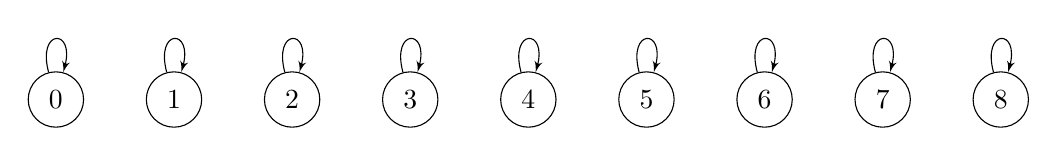
\begin{tikzpicture}
			\node[vertex] (a) at (0, 0) {$0$};
			\node[vertex] (b) at (1.5, 0) {$1$};
			\node[vertex] (c) at (3, 0) {$2$};
			\node[vertex] (d) at (4.5, 0) {$3$};
			\node[vertex] (e) at (6, 0) {$4$};
			\node[vertex] (f) at (7.5, 0) {$5$};
			\node[vertex] (g) at (9, 0) {$6$};
			\node[vertex] (h) at (10.5, 0) {$7$};
			\node[vertex] (i) at (12, 0) {$8$};

			\draw[edge] (a) to[loop above] (a);
			\draw[edge] (b) to[loop above] (b);
			\draw[edge] (c) to[loop above] (c);
			\draw[edge] (d) to[loop above] (d);
			\draw[edge] (e) to[loop above] (e);
			\draw[edge] (f) to[loop above] (f);
			\draw[edge] (g) to[loop above] (g);
			\draw[edge] (h) to[loop above] (h);
			\draw[edge] (i) to[loop above] (i);
		\end{tikzpicture}
	\end{center}

	\vspace{2em}

	Giving us a cycle type of:

	\begin{gather*}
		(1, 1, 1, 1, 1, 1, 1, 1, 1) \\
	\end{gather*}
	
	for $\sigma_{1}$.

	\begin{step}
		Express $\sigma_{2}$ in cycle notation and determine its cycle type.
	\end{step}

	We can once again see that:

	\vspace{2em}

	\begin{tabularx}{\linewidth}{Y | *{9}{Y}}
		$x$ & 0 & 1 & 2 & 3 & 4 & 5 & 6 & 7 & 8 \\
		\hline
		$\sigma_{2}(x)$ & 0 & 2 & 4 & 6 & 8 & 1 & 3 & 5 & 7 \\
	\end{tabularx}

	\vspace{2em}

	represents $\sigma_{2}$ in tabular form. We can use this to graphically represent how $\sigma_{2}$ permutes the elements of $\mathbb{Z}_{9}$, as shown below:

	\vspace{2em}

	\begin{center}
		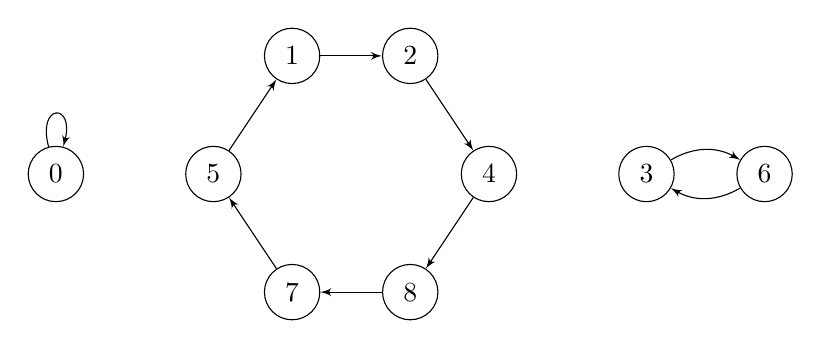
\begin{tikzpicture}
			\node[vertex] (a) at (0, 1.5) {$0$};
			\node[vertex] (b) at (3, 3) {$1$};
			\node[vertex] (c) at (4.5, 3) {$2$};
			\node[vertex] (d) at (5.5, 1.5) {$4$};
			\node[vertex] (e) at (4.5, 0) {$8$};
			\node[vertex] (f) at (3, 0) {$7$};
			\node[vertex] (g) at (2, 1.5) {$5$};
			\node[vertex] (h) at (7.5, 1.5) {$3$};
			\node[vertex] (i) at (9, 1.5) {$6$};

			\draw[edge] (a) to[loop above] (a);
			\draw[edge] (b) to (c);
			\draw[edge] (c) to (d);
			\draw[edge] (d) to (e);
			\draw[edge] (e) to (f);
			\draw[edge] (f) to (g);
			\draw[edge] (g) to (b);
			\draw[edge] (h) to[bend left] (i);
			\draw[edge] (i) to[bend left] (h);
		\end{tikzpicture}
	\end{center}

	\vspace{2em}
	
	Using this, we can quickly ascertain that $\sigma_{2}$ is expressible as:

	\begin{align*}
		\sigma_{2} &= (124875)(36) \\
	\end{align*}

	in cycle notation, giving us a cycle type of:

	\begin{gather*}
		(6, 2, 1) \\
	\end{gather*}

	\begin{step}
		Express $\sigma_{4}$ in cycle notation and determine its cycle type.
	\end{step}

	To avoid beating a dead horse here, this and all future solutions for this part will be presented with considerably sparser commentary. \\

	$\sigma_{4}$'s table is given by:

	\vspace{2em}

	\begin{tabularx}{\linewidth}{Y | *{9}{Y}}
		$x$ & 0 & 1 & 2 & 3 & 4 & 5 & 6 & 7 & 8 \\
		\hline
		$\sigma_{4}(x)$ & 0 & 4 & 8 & 3 & 7 & 2 & 6 & 1 & 5 \\
	\end{tabularx}

	\vspace{2em}

	So, $\sigma_{4}$ looks like:

	\vspace{2em}

	\begin{center}
		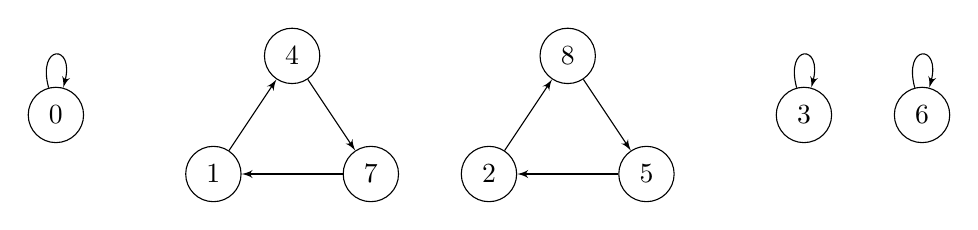
\begin{tikzpicture}
			\node[vertex] (a) at (0, 0.75) {$0$};
			\node[vertex] (b) at (2, 0) {$1$};
			\node[vertex] (c) at (3, 1.5) {$4$};
			\node[vertex] (d) at (4, 0) {$7$};
			\node[vertex] (e) at (5.5, 0) {$2$};
			\node[vertex] (f) at (6.5, 1.5) {$8$};
			\node[vertex] (g) at (7.5, 0) {$5$};
			\node[vertex] (h) at (9.5, 0.75) {$3$};
			\node[vertex] (i) at (11, 0.75) {$6$};

			\draw[edge] (a) to[loop above] (a);
			\draw[edge] (b) to (c);
			\draw[edge] (c) to (d);
			\draw[edge] (d) to (b);
			\draw[edge] (e) to (f);
			\draw[edge] (f) to (g);
			\draw[edge] (g) to (e);
			\draw[edge] (h) to[loop above] (i);
			\draw[edge] (i) to[loop above] (h);
		\end{tikzpicture}
	\end{center}

	\vspace{2em}

	Giving that:

	\begin{align*}
		\sigma_{4} &= (147)(285) \\
	\end{align*}

	And a cycle type of:

	\begin{gather*}
		(3, 3, 1, 1, 1) \\
	\end{gather*}

	\begin{step}
		Express $\sigma_{5}$ in cycle notation and determine its cycle type.
	\end{step}

	$\sigma_{5}$'s table is given by:

	\vspace{2em}

	\begin{tabularx}{\linewidth}{Y | *{9}{Y}}
		$x$ & 0 & 1 & 2 & 3 & 4 & 5 & 6 & 7 & 8 \\
		\hline
		$\sigma_{5}(x)$ & 0 & 5 & 1 & 6 & 2 & 7 & 3 & 8 & 4 \\
	\end{tabularx}

	\vspace{2em}

	So, $\sigma_{5}$ looks like:

	\vspace{2em}

	\begin{center}
		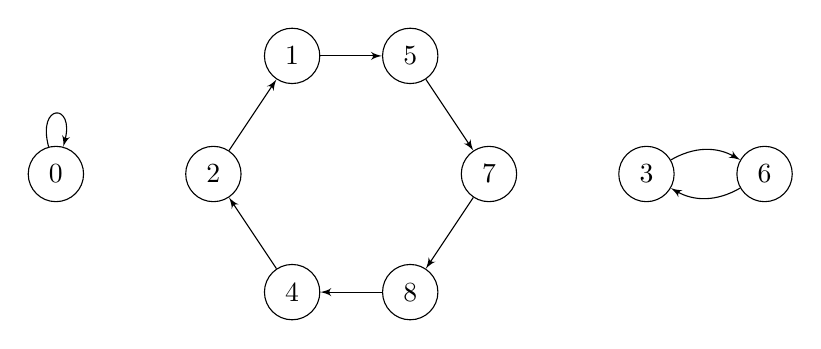
\begin{tikzpicture}
			\node[vertex] (a) at (0, 1.5) {$0$};
			\node[vertex] (b) at (3, 3) {$1$};
			\node[vertex] (c) at (4.5, 3) {$5$};
			\node[vertex] (d) at (5.5, 1.5) {$7$};
			\node[vertex] (e) at (4.5, 0) {$8$};
			\node[vertex] (f) at (3, 0) {$4$};
			\node[vertex] (g) at (2, 1.5) {$2$};
			\node[vertex] (h) at (7.5, 1.5) {$3$};
			\node[vertex] (i) at (9, 1.5) {$6$};

			\draw[edge] (a) to[loop above] (a);
			\draw[edge] (b) to (c);
			\draw[edge] (c) to (d);
			\draw[edge] (d) to (e);
			\draw[edge] (e) to (f);
			\draw[edge] (f) to (g);
			\draw[edge] (g) to (b);
			\draw[edge] (h) to[bend left] (i);
			\draw[edge] (i) to[bend left] (h);
		\end{tikzpicture}
	\end{center}

	\vspace{2em}

	Giving that:

	\begin{align*}
		\sigma_{5} &= (157842)(36) \\
	\end{align*}

	And a cycle type of:

	\begin{gather*}
		(6, 2, 1) \\
	\end{gather*}

	As a side note, notice that since 2 and 5 are inverses of each other in $\mathbb{Z^{\times}}_{9}$, they have the same cycle type but inverted cycles!

	\begin{step}
		Express $\sigma_{7}$ in cycle notation and determine its cycle type.
	\end{step}

	$\sigma_{7}$'s table is given by:

	\vspace{2em}

	\begin{tabularx}{\linewidth}{Y | *{9}{Y}}
		$x$ & 0 & 1 & 2 & 3 & 4 & 5 & 6 & 7 & 8 \\
		\hline
		$\sigma_{7}(x)$ & 0 & 7 & 5 & 3 & 1 & 8 & 6 & 4 & 2 \\
	\end{tabularx}

	\vspace{2em}

	So, $\sigma_{7}$ looks like:

	\vspace{2em}

	\begin{center}
		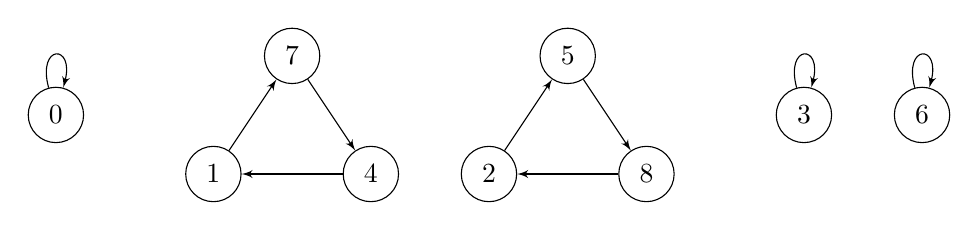
\begin{tikzpicture}
			\node[vertex] (a) at (0, 0.75) {$0$};
			\node[vertex] (b) at (2, 0) {$1$};
			\node[vertex] (c) at (3, 1.5) {$7$};
			\node[vertex] (d) at (4, 0) {$4$};
			\node[vertex] (e) at (5.5, 0) {$2$};
			\node[vertex] (f) at (6.5, 1.5) {$5$};
			\node[vertex] (g) at (7.5, 0) {$8$};
			\node[vertex] (h) at (9.5, 0.75) {$3$};
			\node[vertex] (i) at (11, 0.75) {$6$};

			\draw[edge] (a) to[loop above] (a);
			\draw[edge] (b) to (c);
			\draw[edge] (c) to (d);
			\draw[edge] (d) to (b);
			\draw[edge] (e) to (f);
			\draw[edge] (f) to (g);
			\draw[edge] (g) to (e);
			\draw[edge] (h) to[loop above] (i);
			\draw[edge] (i) to[loop above] (h);
		\end{tikzpicture}
	\end{center}

	\vspace{2em}

	Giving that:

	\begin{align*}
		\sigma_{7} &= (174)(258) \\
	\end{align*}

	And a cycle type of:

	\begin{gather*}
		(3, 3, 1, 1, 1) \\
	\end{gather*}

	\begin{step}
		Express $\sigma_{8}$ in cycle notation and determine its cycle type.
	\end{step}

	Finally getting to the last permutation, $\sigma_{8}$'s table is given by:

	\vspace{2em}

	\begin{tabularx}{\linewidth}{Y | *{9}{Y}}
		$x$ & 0 & 1 & 2 & 3 & 4 & 5 & 6 & 7 & 8 \\
		\hline
		$\sigma_{8}(x)$ & 0 & 8 & 7 & 6 & 5 & 4 & 3 & 2 & 1 \\
	\end{tabularx}

	\vspace{2em}

	So, $\sigma_{8}$ looks like:

	\vspace{2em}

	\begin{center}
		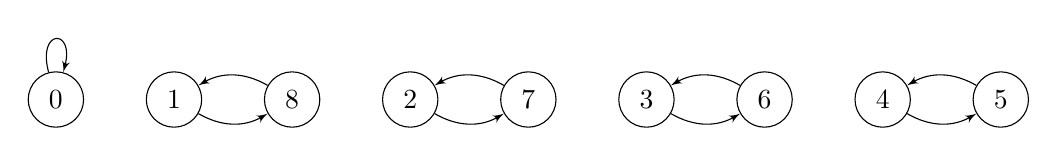
\begin{tikzpicture}
			\node[vertex] (a) at (0, 0) {$0$};
			\node[vertex] (b) at (1.5, 0) {$1$};
			\node[vertex] (c) at (3, 0) {$8$};
			\node[vertex] (d) at (4.5, 0) {$2$};
			\node[vertex] (e) at (6, 0) {$7$};
			\node[vertex] (f) at (7.5, 0) {$3$};
			\node[vertex] (g) at (9, 0) {$6$};
			\node[vertex] (h) at (10.5, 0) {$4$};
			\node[vertex] (i) at (12, 0) {$5$};

			\draw[edge] (a) to[loop above] (a);
			\draw[edge] (b) to[bend right] (c);
			\draw[edge] (c) to[bend right] (b);
			\draw[edge] (d) to[bend right] (e);
			\draw[edge] (e) to[bend right] (d);
			\draw[edge] (f) to[bend right] (g);
			\draw[edge] (g) to[bend right] (f);
			\draw[edge] (h) to[bend right] (i);
			\draw[edge] (i) to[bend right] (h);
		\end{tikzpicture}
	\end{center}

	\vspace{2em}

	Giving that:

	\begin{align*}
		\sigma_{8} &= (18)(27)(36)(45) \\
	\end{align*}

	And a cycle type of:

	\begin{gather*}
		(2, 2, 2, 2, 1) \\
	\end{gather*}
\end{solution}

\begin{problem}
	Let $G$ be a set, and let $\ast$ be an associative binary operator on $G$ with identity element $e \in G$. Suppose that for each $x \in G$, there exists $y \in G$ such that $x \ast y = e$. Prove that $G$ is a group under $\ast$. \\

	\emph{Note:} In your proof, make sure to clearly indicate where each property is used (I.E., Associativity, identity, etc.).
\end{problem}

\begin{solution}
	We know that for $G$ to be a group under $\ast$:
	\begin{enumerate}
		\item $\ast$ must be a binary operator over $G$.
		\item $\ast$ must be associative over $G$.
		\item $\ast$ must have an identity element in $G$.
		\item Every element in $G$ must have an inverse in $G$ with respect to $\ast$. \\
	\end{enumerate}

	The question itself already grants to us that $\ast$ over $G$ satisfies criteria 1 through 3, and so we need only verify that $\ast$ also satisfies criterion 4 to conclude that $(G, \ast)$ is a group. \\

	In the definition of group we use in this course, we require that every element $x \in G$ must have some element $y \in G$ (known as an inverse of $x$) such that $x \ast y = y \ast x = e$, where $e$ is the identity element in $G$. However, the question grants us only that for every such $x$, there exists some $y \in G$ satisfying $x \ast y = e$. \\

	Notice however, that since $y \in G$ as well, there must similarly exist some $z \in G$ for which $y \ast z = e$. And so, since:

	\begin{align*}
		x \ast y &= e &&\text{(Since $y$ is a right inverse of $x$)} \\
		\implies (x \ast y) \ast z &= e \ast z &&\text{(Multiplying both sides by $z$ on the right)} \\
		\implies x \ast (y \ast z) &= e \ast z &&\text{(By associativity of $\ast$ over $G$)} \\
		\implies x \ast e &= e \ast z &&\text{(Since $z$ is a right inverse of $y$)} \\
		\implies x &= e \ast z &&\text{(By definition of the identity)} \\
		\implies x &= z &&\text{(By definition of the identity)} \\
	\end{align*}

	We get that:

	\begin{align*}
		y \ast z &= e &&\text{(Since $z$ is a right identity of $y$)} \\
		\implies y \ast x &= e &&\text{(Since $x = z$ from earlier implications)} \\
	\end{align*}

	And so, since $x \ast y = y \ast x = e$ and $x \in G$ was arbitrary, we have that every element of $G$ has an inverse in $G$ with respect to $\ast$. And thus, since $(G, \ast)$ satisfies all four criteria necessary to be a group outlined earlier, $G$ does indeed constitute a group under $\ast$.
\end{solution}

\begin{problem}
	Let $G$ be a group. Suppose that $g^{2} = 1$ for all $g \in G$. Prove that $G$ is an abelian group.
\end{problem}

\begin{solution}
	Let $x, y \in G$ be arbitrary. We know by definition that for $G$ to be an abelian group, that it must satisfy:

	\begin{align*}
		xy &= yx \\
	\end{align*}

	for all such $x$ and $y$. \\

	Since the question already gives to us that $G$ is a group, we know that it must be closed under its group operation, and so $xy$ must belong to $G$. The question also grants us that every element in $G$ composed with itself equals the identity element (or in other words, that each element is its own inverse), and so it follows not only that $x^{2} = 1$ and $y^{2} = 1$, but $(xy)^{2} = 1$ as well. Putting all of this together, this means that:

	\begin{align*}
		(xy)^{2} &= 1 &&\text{(Since $(xy)^{2} = 1$)} \\
		\implies (xy)(xy) &= 1 &&\text{(By definition of $(xy)^{2}$)} \\
		\implies x(y(xy)) &= 1 &&\text{(By associativity)} \\
		\implies x^{2}(y(xy)) &= x &&\text{(Multiplying both sides by $x$ on the left)} \\
		\implies 1(y(xy)) &= 1(x) &&\text{(Since $x^{2} = 1$)} \\
		\implies y(xy) &= x &&\text{(By definition of identity)} \\
		\implies y^{2}(xy) &= yx &&\text{(Multplying both sides by $y$ on the left)} \\
		\implies 1(xy) &= yx &&\text{(Since $y^{2} = 1$)} \\
		\implies xy &= yx &&\text{(By definition of identity)} \\
	\end{align*}

	And so $G$ is indeed abelian!
\end{solution}






\ifdefined\iscombined
	\newpage
\else
	\end{document}
\fi
